% !TeX spellcheck = da_DK
\chapter{Kroppens balance}\label{app-Balance}
%Apopleksipatienter oplever ofte problemer med balancen, da den ofte er nedsat eller slet ikke funktionsdygtig af forskellige årsager. \cite{Karnath2003} 
Proprioceptorer og sansereceptorer hjælper kroppen med balancen. Proprioceptorerne kontrollerer muskler, sener og leddenes position, hvorimod sansereceptorer er en bestemt slags celler, som f.eks. er placeret i ørerne og øjnene. \cite{Martini2012} Disse celler sender balanceinformationer til CNS og encephalon. Sansereceptorerne opfanger indtryk fra sanserne, som omsættes til bestemte signaler, der sendes til områder i cerebral cortex, cerebellum og centre i hele hjernestammen. Her bearbejdes informationen, hvorefter den korrekte fysiske position af kroppen og dens lemmer konkluderes. Når encephalon har bearbejdet indtrykkene, udsender den nerveimpulser til skeletmuskulaturen om at foretage jævne og koordinerede bevægelser, hvorved kropsbalancen opretholdes.\cite{Martini2012}

Øjet opfanger lys og er med til orienteringen af kroppen og dens lemmer. Hårceller i øret registrerer f.eks. hovedets bevægelser vha. tyngdekraften. Selvom et balanceorgan er ude af funktion, er kroppen stadig i stand til at opretholde balancen ved hjælp fra andre balanceorganer. Det er til gengæld vanskeligt for kroppen at opretholde balancen, hvis de behandlende centre i encephalon bliver skadet, som det kan ske ved apopleksipatienter. \cite{Martini2012} \\

\section{Ørets bidrag til balancen}
Øret består overordnet af tre dele; det ydre øre, mellemøret og det indre øre, som kan ses på \figref{Oeret}. 
\begin{figure}[H]
	\centering
	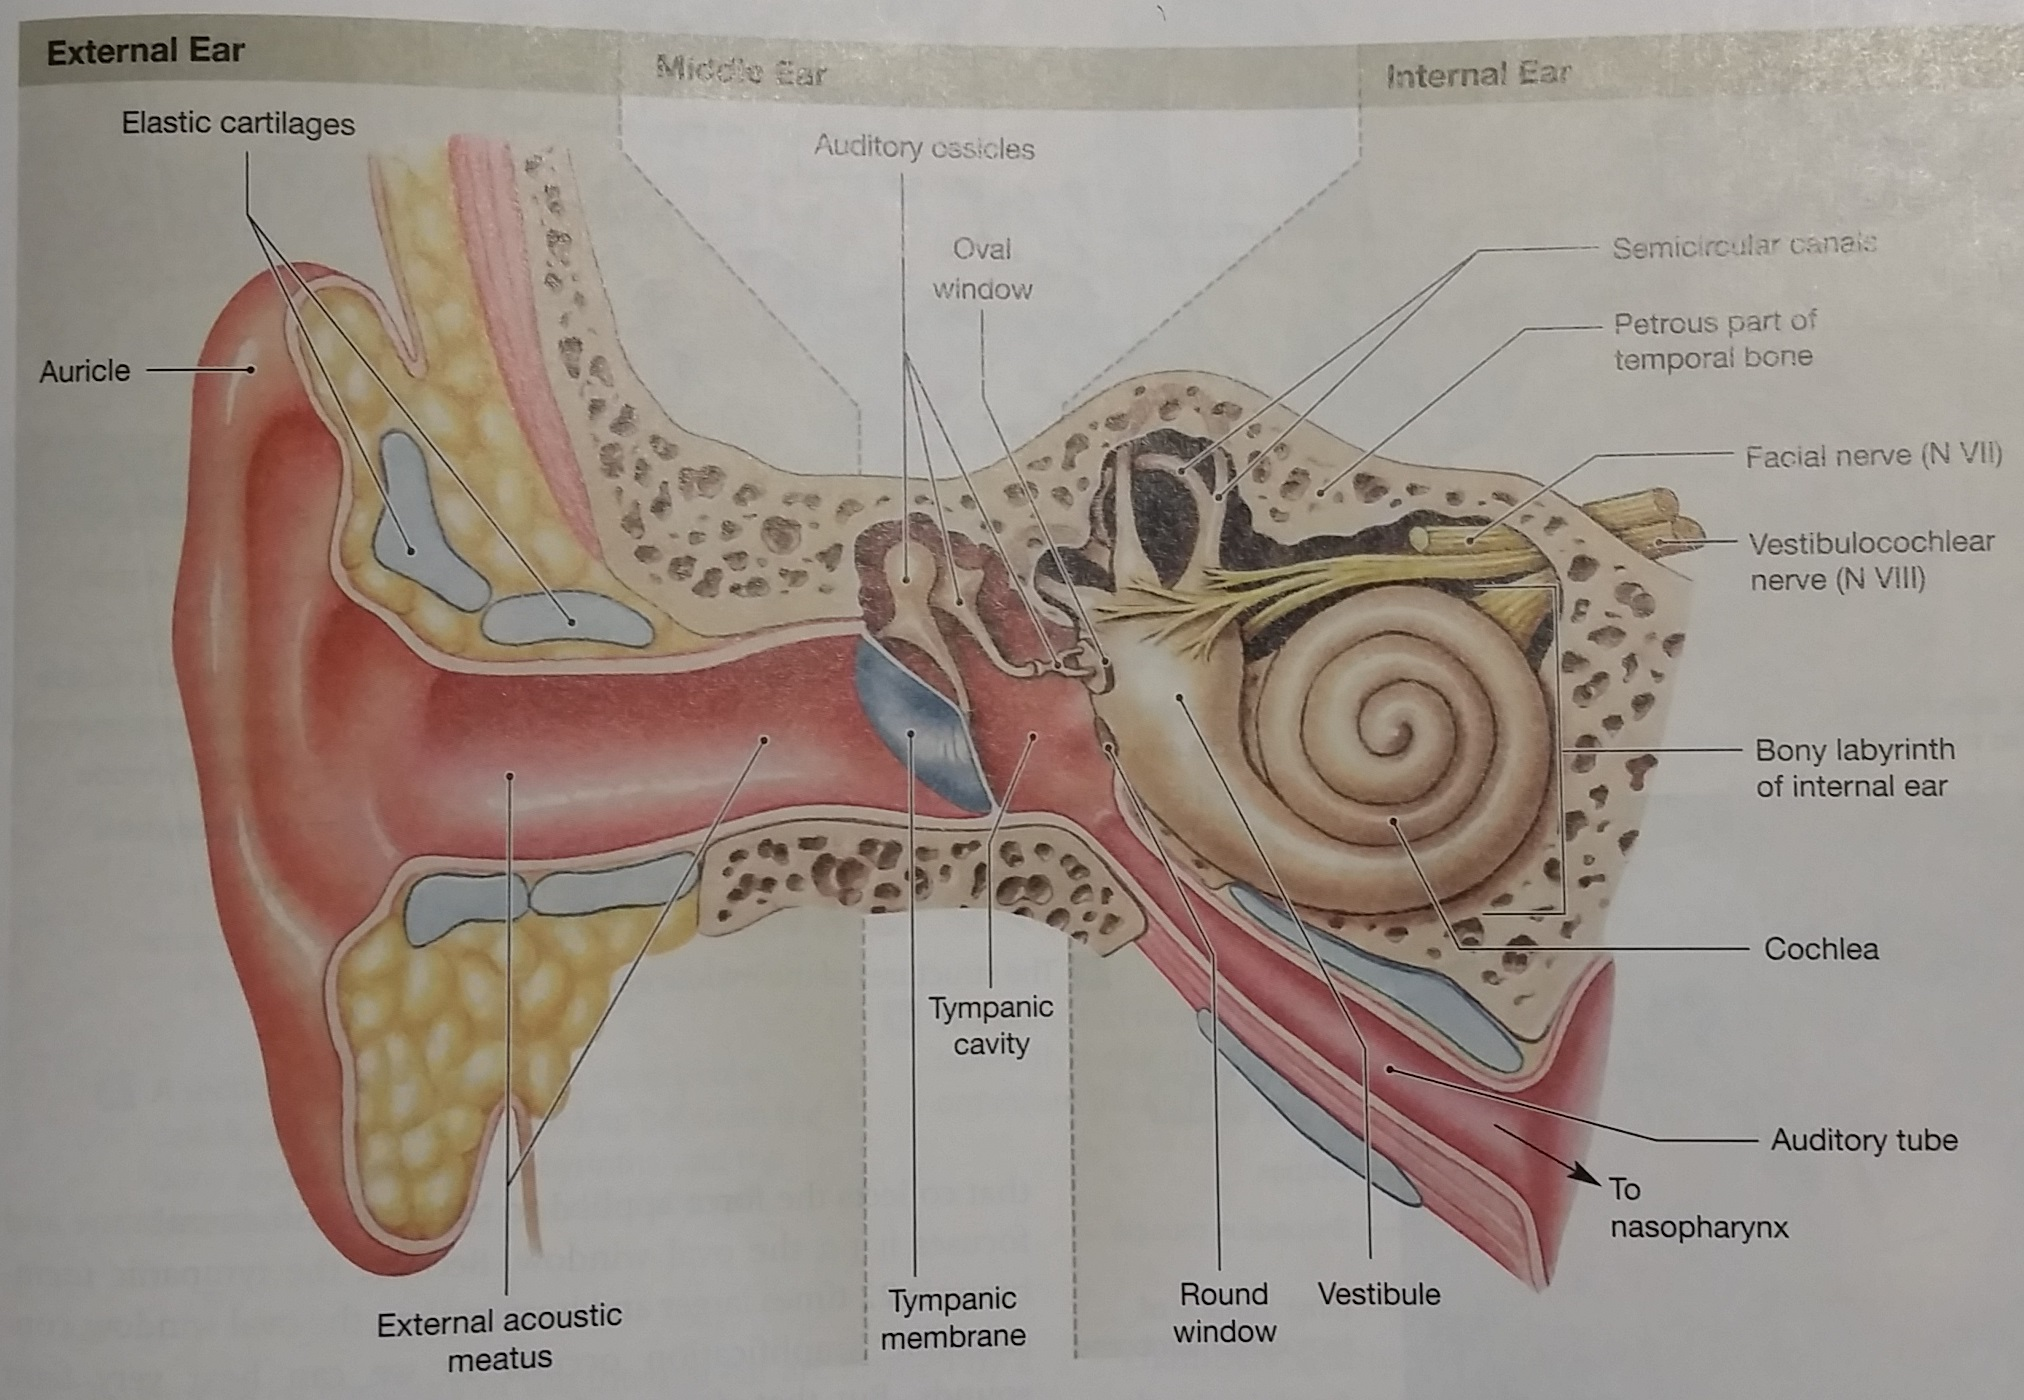
\includegraphics[scale=0.75]{figures/bProblemanalyse/Oerets-anatomi.jpg}
	\caption{På figuren ses ørets anatomiske opbygning \cite{Martini2012}.}
	\label{Oeret}
\end{figure}
Det indre øre er med til at kontrollere balancen vha. hårcellerne, som sættes i bevægelse. Det ydre øre modtager trykbølger, som sætter trommehinden i svingninger. Disse transporteres af mellemørets knogler, der forstærker svingningerne. Væsken i mellemøret modtager svingningerne fra knoglerne, hvilket sætter væsken i bevægelse. Denne bevægelse trækker i hårcellerne, og der skabes derved et aktionspotentiale. I det indre øre findes et netværk af sammenhængende væskeholdige kanaler, som er indkapslet i knoglen. Det er i disse kanaler receptorerne sidder. Det indre øre kan opdeles i tre undergrupper; vestibulen, øresneglen og buegangen. De centrale dele, der er relateret til balancen, er vestibulen og buegangen, hvorimod øresneglen kun bidrager til hørelsen. \cite{Martini2012}

Vestibulen består af to membransække; sacculen og utriclen, der opfanger sanseindtryk vedrørende tyngdekraft og lineær acceleration. Buegangens sansereceptorer opfanger stimuli omkring hovedets bevægelse, og hvor hurtigt bevægelsen foregår. Sansereceptorerne er placeret i buegangens tre væskefyldte knoglekanaler ved ampulla, der er forbundet til utriclen. Hårcellerne er kun aktive, når kroppen er i bevægelse ved at videregive information vedrørende hovedets bevægelse ift. tyngdekraften. Når hovedet er i bevægelse, sættes væsken i kanalerne også i bevægelse således, at væskebevægelser i den ene retning stimulerer hårcellerne, mens bevægelser i den modsatte retning forhindrer dem. For at få mest mulig information angående hovedets position, stimuleres de tre buegange af forskellige hovedbevægelser. Bevægelsesinformationerne sendes via vestibulocochlearnerven, der sender både information vedrørende balancen og hørelsen til encephalon i området mellem pons og medulla oblongata. \cite{Martini2012}    

\section{Øjets bidrag til balancen}
Synet er en central faktor for, hvordan encephalon holdes informeret omkring kroppens balance og generelle orientering. Dette gøres ved at give et indtryk af, hvordan kroppen og dens lemmer er placeret ift. omgivelserne. \cite{Schulmann1987} Øjet har tre hinder; fibrøs hinde, uvea og retina, som kan ses på \figref{Oejet}.
\begin{figure}[H]
	\centering
	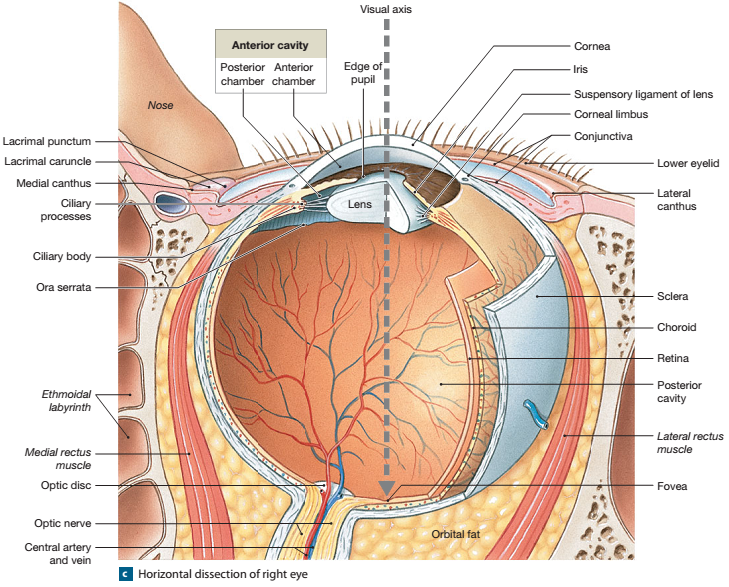
\includegraphics[scale=0.75]{figures/bProblemanalyse/Oejets-anatomi.png}
	\caption{På figuren ses øjets anatomisk opbygning. \cite{Martini2012}}
	\label{Oejet}
\end{figure}
Den fibrøse hinde\fxnote{NTK: hornhinden} er den yderste, som beskytter og støtter øjet. Den midterste hinde, kaldet uvea, indeholder blod og lymfekar samt regulerer mængden af lys, der kommer ind i øjet. Retina\fxnote{NTK: nethinden} er den inderste hinde, som er placeret bagerst i øjet. Den består af en pigmentdel og en indre neuraldel. Den neurale del indeholder fotoreceptorer, bestående af stave og tappe. Stave er følsomme overfor skarpt lys og gør det muligt at se i mørke. Tappe er følsomme overfor farvers bølgelængde, hvilket giver farvesyn. Pigmentdelen absorberer lys, der passerer gennem den neurale del og gør, at lyset ikke har mulighed for at reflektere tilbage. Foto- og lysreceptorerne konverterer lyset fra omgivelserne til elektrisk nervesignal, der giver information omkring det objekt, der betragtes, herunder dets størrelse, form og bevægelser. Informationerne processeres således, at horisontale celler lokaliserer områdets størrelse. Hvis der er kommet tilstrækkeligt med lys ind, sendes informationen først til bipolære celler herefter via synsnerven til det visuelle cortex, hvor informationen bearbejdes. \cite{Martini2012}     

\section{Proprioceptorerne og skeletmuskulaturens bidrag til balancen}
Proprioceptorer monitorerer leddenes position, muskelkontraktioners tilstand, samt spændingen i ledbånd og sener. Disse er placeret i skeletmuskulaturen. Informationerne sendes via nervesignaler til medulla spinalis og herfra igennem CNS til cerebellum. Proprioceptorer inddeles i tre overordnet grupper; muskelspindlere, golgi-sene organer og receptorer i ledkapsler. \cite{Martini2012}

Muskelspindlere styrer og kontrollerer ændringer af muskellængder og kan udløse en strækrefleks. Den sensoriske nerve er forbundet centralt på muskelspindleren, hvor den kontinuert sender sensoriske impulser til CNS. Hvis den sensoriske nerve modtager stimuli, i form af stræk, vil den motoriske nerve på muskelspindleren blive stimuleret. Stimulation af den motoriske nerve vil forkorte musklens længde. Nogle strækreflekser er holdningsreflekser, som hjælper til at holde balancen. I stående position kræves der et samarbejde mellem forskellige muskelgrupper for at forblive stående. Dette ses f.eks. hvis kroppen lænes forover, vil strækreflekserne i læggene blive aktiveret og kontraherer. Derved vil kroppen læne sig bagud og igen stå i en opret position. Hvis der sker en overkompensation fra lægmusklerne og kroppen læner sig for meget bagud, vil strækreflekser i skinnebenet og lårene aktiveres. Derved vil kroppen læne sig forover igen. Kroppen foretager mange af disse ubevidste korrektioner. \cite{Martini2012}   %(Se Martini 9th side 438 under "monosynaptic reflexes")

Golgi-sene organer sidder i en kløft\fxnote{NTK: kaldes junction på engelsk} mellem skeletmusklen og tilhørende sene. Dendritterne fra golgi-sene organet kobler sig på den nærmeste sene og stimuleres af spændingen i denne, hvorved den eksterne spænding i en muskelkontraktion bliver målt. \cite{Martini2012} 

Ledkapsler er fyldt med frie nerveender, som kaldes receptorer. Disse receptorer detekterer tryk, spænding og bevægelse i leddet. \cite{Martini2012}    \\
Det er en lille del, af den information proprioceptererne sender, der opfanges af bevidstheden, eftersom størstedelen foregår på et underbevidst niveau. \cite{Martini2012} \\


%Golgi seneorganer (Se Martini 9th side 501 under 15-3 propriocetor) %Receptorer i ledkapsler (Se Martini 9th side 501 under 15-3 propriocetor)

%\subsection{Apopleksi og balance}
%Balancen er styrer flere steder i kroppen og er med til at beskytte kroppen mod f.eks. faldulykker, ved at sikre at kroppen og den lemmer bevæger sig i kontrollerede og jævne bevægelser. Kroppen opretholder balancen ved at bruge ørerne, øjne og proprioceptorer i skeletmuskulaturen. Proprioceptorerne kontrollerer muskler, sener og leds position. Øjne opfanger lys og er med til orienteringen af kroppen og dens lemmer og hårceller i øret register hoveds bevægelser ved hjælp af tyngdekraften. Selvom et balanceorgan er ude af funktion er kroppen stadig i stand til at opretholde balancen ved hjælp fra andre balanceorganer. Det er til gengæld svære for kroppen at opretholde balancen hvis centrene i hjerne, som behandler den information, som kommer fra balanceorganerne, bliver skadet, som det kan ske ved apopleksi patienter. \cite{Martini2012}
% [1] – Martini, Frederic H and others. Fundamentals of Anatomy & Physiology (Kapitel:13, 14, 15, 17 ). 2012. Pearson. 
% [2] - Karnath2003